\chapter[Explorer16 Board]{Explorer16 Board}

\section{Introduction}

This chapter describes the support done in \ee\ for the
Microchip Explorer16 Board (see Figure \ref{fig:explorer16}).

\begin{figure}
  \begin{center}
    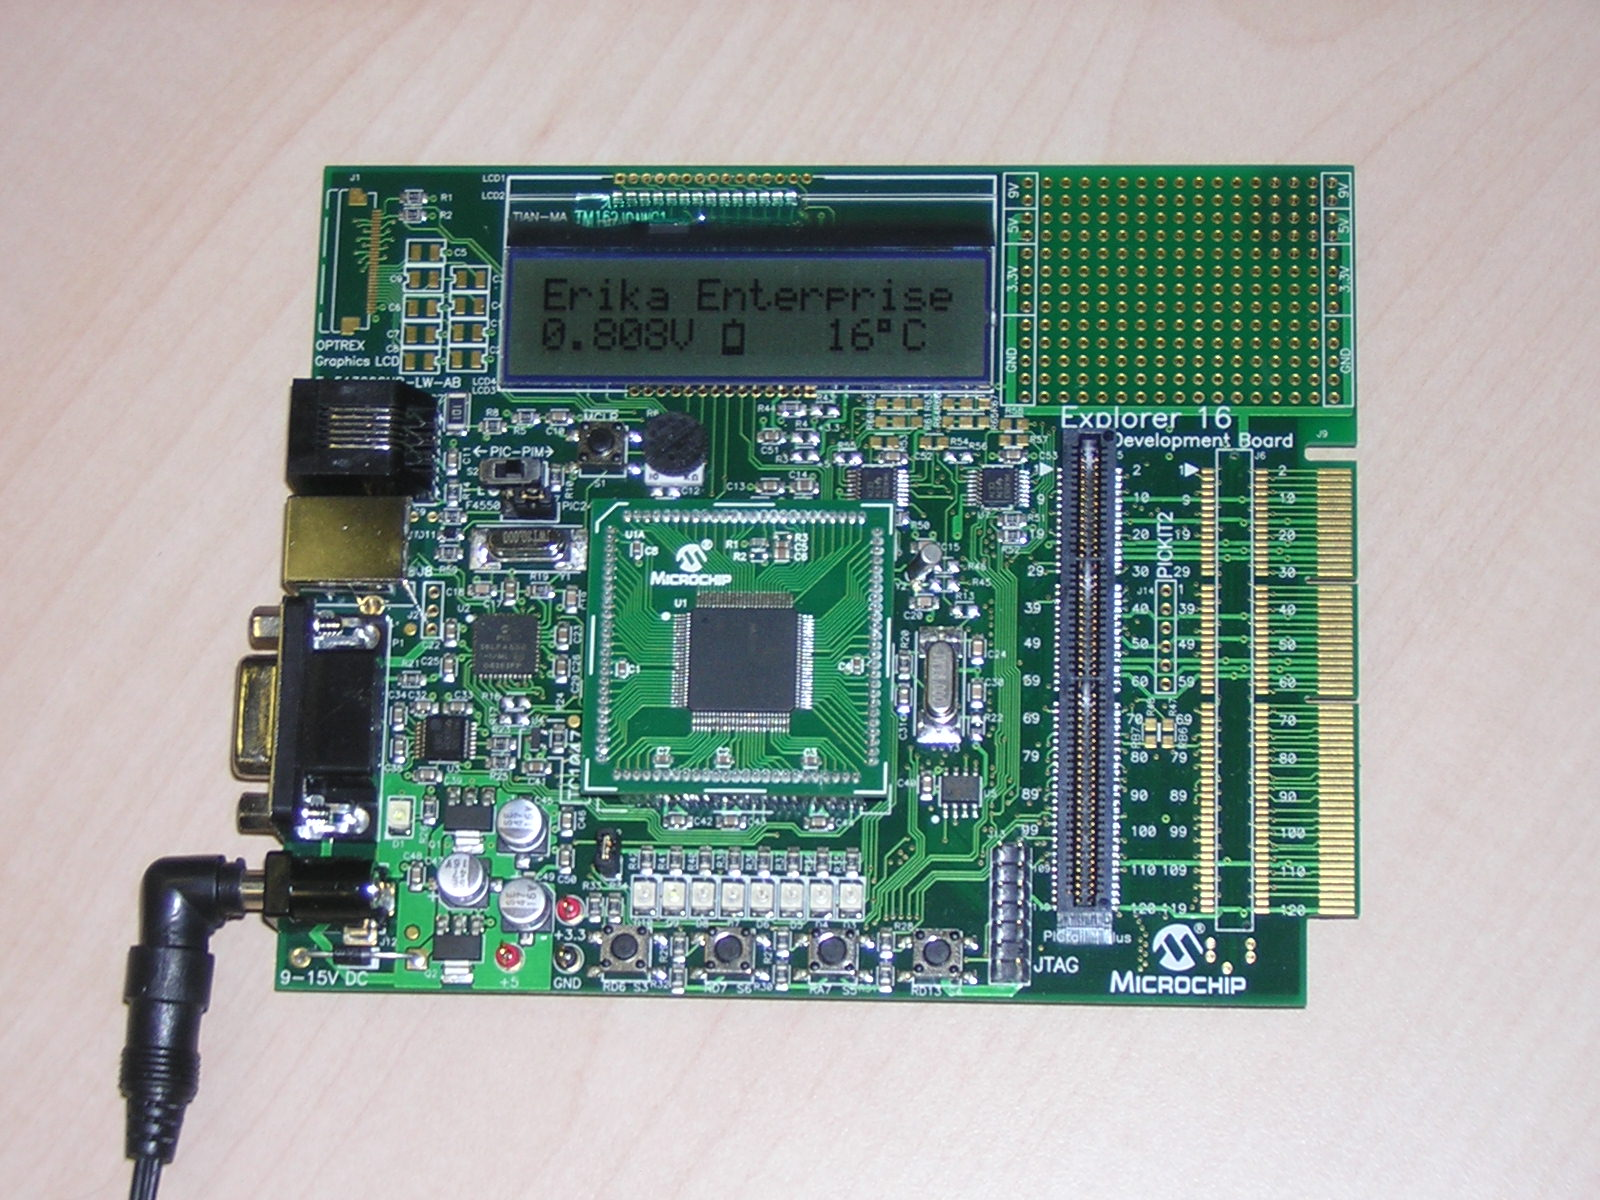
\includegraphics[width=6cm, bb=0 0 1600 1200]{images/explorer16running.jpg}
  \end{center}
  \caption{The Microchip Explorer 16 board running \ee.}
  \label{fig:explorer16}
\end{figure}

The Explorer 16 is a low cost, efficient development board produced by
Microchip hosting an alpha-numeric 16 x 2 LCD display, with interfaces
to MPLAB ICD 2, USB, and RS-232 \cite{MicrochipExplorer16}.

To configure the usage of the Explorer 16 Board, the user has to specify an
appropriate \const{BOARD_DATA}, as in the following example:

\begin{lstlisting}
  ...
  BOARD_DATA = MICROCHIP_EXPLORER16 {
    ...
  }
  ...
\end{lstlisting}

The Explorer 16 board supports a set of devices which are directly
mounted on it. These devices can be configured by adding attributes
inside the \const{BOARD_DATA} section.

The supported devices and the API functions needed to use them are
described in the following sections.

The current version of the board support for Flex supports both the
\dspic\ model 33FJ256GP710 and the PIC24 model 24FJ128GA010.


% -------------------------------------------------------------------

\section{Buttons}

The Explorer 16 Board has a set of four buttons attached to GPIO pins
of the microcontroller. To use the buttons on the Explorer 16 Board, the
developer should specify the \const{USEBUTTONS} attribute as TRUE, as
in the following example:

\begin{lstlisting}
  ...
  BOARD_DATA = MICROCHIP_EXPLORER16 {
    USEBUTTONS = TRUE;
    ...
  }
  ...
\end{lstlisting}

The following subsections will describe the functions available to
control the Explorer 16 buttons.

\begin{function_nopb2}{EE\_buttons\_init}{EE_buttons_init}
  \synopsis{void EE_buttons_init( void (*isr_callback)(void), EE_UINT8 mask );}
  
  \begin{fundescription}
    The function configures the GPIO pins used by the buttons. Buttons
    can be configured to be controlled only by using polling functions
    (no \fn{isr_callback} is specified), or can be configured to raise
    an interrupt (if \fn{isr_callback} is specified).

    When the \fn{isr_callback} is specified, the \fn{mask} parameter
    is used to control for which buttons the interrupt will be
    generated.
  \end{fundescription}
  
  \begin{funparameters}
    \fpar{isr_callback}{The function is called inside an ISR2 upon a
      button press.}

    \fpar{mask}{If \fn{isr_callback} is specified, then this parameter
      controls which buttons will generate an interrupt request. In
      particular, bit \const{0x01} is used for button S3, bit
      \const{0x02} is used for button S4, bit \const{0x04} is used for
      button S5, bit \const{0x08} is used for button S6.}
  \end{funparameters}
  
  \begin{funreturn}
    \fret{void}{The function does not return a value.}
  \end{funreturn}
  
%  \begin{funconformance}
%  \end{funconformance}
\end{function_nopb2}

\begin{function_nopb2}{EE\_button\_get\_S3}{EE_button_get_S3}
  \synopsis{EE_UINT8 EE_button_get_S3(void);}
  
  \begin{fundescription}
    The function returns the status of the button number S3.
  \end{fundescription}
  
%  \begin{funparameters}
%    \fpar{none}{None in this function.}
%  \end{funparameters}
  
  \begin{funreturn}
    \fret{unsigned char}{1 of the button is pressed, 0 otherwise.}
  \end{funreturn}
  
%  \begin{funconformance}
%  \end{funconformance}
\end{function_nopb2}

\begin{function_nopb2}{EE\_button\_get\_S4}{EE_button_get_S4}
  \synopsis{EE_UINT8 EE_button_get_S4(void);}
  
  \begin{fundescription}
    The function returns the status of the button number S4.
  \end{fundescription}
  
%  \begin{funparameters}
%    \fpar{none}{None in this function.}
%  \end{funparameters}
  
  \begin{funreturn}
    \fret{unsigned char}{1 of the button is pressed, 0 otherwise.}
  \end{funreturn}
  
%  \begin{funconformance}
%  \end{funconformance}
\end{function_nopb2}

\begin{function_nopb2}{EE\_button\_get\_S5}{EE_button_get_S5}
  \synopsis{EE_UINT8 EE_button_get_S5(void);}
  
  \begin{fundescription}
    The function returns the status of the button number S5.
  \end{fundescription}
  
%  \begin{funparameters}
%    \fpar{none}{None in this function.}
%  \end{funparameters}
  
  \begin{funreturn}
    \fret{unsigned char}{1 of the button is pressed, 0 otherwise.}
  \end{funreturn}
  
%  \begin{funconformance}
%  \end{funconformance}
\end{function_nopb2}

\begin{function_nopb2}{EE\_button\_get\_S6}{EE_button_get_S6}
  \synopsis{EE_UINT8 EE_button_get_S6(void);}
  
  \begin{fundescription}
    The function returns the status of the button number S6.
  \end{fundescription}
  
%  \begin{funparameters}
%    \fpar{none}{None in this function.}
%  \end{funparameters}
  
  \begin{funreturn}
    \fret{unsigned char}{1 of the button is pressed, 0 otherwise.}
  \end{funreturn}
  
%  \begin{funconformance}
%  \end{funconformance}
\end{function_nopb2}




% -------------------------------------------------------------------

\section{LEDs}

The Explorer 16 Board has a set of 8 LEDs attached to the GPIO pins of the
microcontroller. To use the LEDs on the Explorer 16 Board, the
developer should specify the \const{USELEDS} attribute as TRUE, as in
the following example:

\begin{lstlisting}
  ...
  BOARD_DATA = MICROCHIP_EXPLORER16 {
    USELEDS = TRUE;
    ...
  }
  ...
\end{lstlisting}

The following subsections will describe the functions available to
control the Explorer 16 LEDs.

\begin{function_nopb2}{EE\_leds\_init}{EE_leds_init:explorer16}
  \synopsis{void EE_leds_init(void);}
  
  \begin{fundescription}
    The function configures the GPIO pins. The LEDs start turned off.
  \end{fundescription}
  
%  \begin{funparameters}
%    \fpar{none}{None in this function.}
%  \end{funparameters}
  
%  \begin{funreturn}
%    \fret{void}{The function does not return a value.}
%  \end{funreturn}
  
%  \begin{funconformance}
%  \end{funconformance}
\end{function_nopb2}

\begin{function_nopb2}{EE\_leds\_on}{EE_leds_on}
  \synopsis{void EE_leds_on(void);}
  
  \begin{fundescription}
    The function turns on all the LEDs.
  \end{fundescription}
  
%  \begin{funparameters}
%    \fpar{none}{None in this function.}
%  \end{funparameters}
  
%  \begin{funreturn}
%    \fret{void}{The function does not return a value.}
%  \end{funreturn}
  
%  \begin{funconformance}
%  \end{funconformance}
\end{function_nopb2}

\begin{function_nopb2}{EE\_leds\_off}{EE_leds_off}
  \synopsis{void EE_leds_off(void);}
  
  \begin{fundescription}
    The function turns off all the LEDs.
  \end{fundescription}
  
%  \begin{funparameters}
%    \fpar{none}{None in this function.}
%  \end{funparameters}
  
%  \begin{funreturn}
%    \fret{void}{The function does not return a value.}
%  \end{funreturn}
  
%  \begin{funconformance}
%  \end{funconformance}
\end{function_nopb2}


\begin{function_nopb2}{EE\_led\_on}{EE_led_on:explorer16}
  \synopsis{void EE_led_on(void);}
  
  \begin{fundescription}
    The function turns on LED 3 (which is the first led on the board).
  \end{fundescription}
  
%  \begin{funparameters}
%    \fpar{none}{None in this function.}
%  \end{funparameters}
  
%  \begin{funreturn}
%    \fret{void}{The function does not return a value.}
%  \end{funreturn}
  
%  \begin{funconformance}
%  \end{funconformance}
\end{function_nopb2}

\begin{function_nopb2}{EE\_led\_off}{EE_led_off:explorer16}
  \synopsis{void EE_led_off(void);}
  
  \begin{fundescription}
    The function turns off LED 3 (which is the first led on the board).
  \end{fundescription}
  
%  \begin{funparameters}
%    \fpar{none}{None in this function.}
%  \end{funparameters}
  
%  \begin{funreturn}
%    \fret{void}{The function does not return a value.}
%  \end{funreturn}
  
%  \begin{funconformance}
%  \end{funconformance}
\end{function_nopb2}

\begin{function_nopb2}{EE\_led\_3\_on}{EE_led_3_on}
  \synopsis{void EE_led_3_on(void);}
  
  \begin{fundescription}
    The function turns on LED 3.
  \end{fundescription}
  
%  \begin{funparameters}
%    \fpar{none}{None in this function.}
%  \end{funparameters}
  
%  \begin{funreturn}
%    \fret{void}{The function does not return a value.}
%  \end{funreturn}
  
%  \begin{funconformance}
%  \end{funconformance}
\end{function_nopb2}

\begin{function_nopb2}{EE\_led\_3\_off}{EE_led_3_off}
  \synopsis{void EE_led_3_off(void);}
  
  \begin{fundescription}
    The function turns off LED 3.
  \end{fundescription}
  
%  \begin{funparameters}
%    \fpar{none}{None in this function.}
%  \end{funparameters}
  
%  \begin{funreturn}
%    \fret{void}{The function does not return a value.}
%  \end{funreturn}
  
%  \begin{funconformance}
%  \end{funconformance}
\end{function_nopb2}

\begin{function_nopb2}{EE\_led\_4\_on}{EE_led_4_on}
  \synopsis{void EE_led_4_on(void);}
  
  \begin{fundescription}
    The function turns on LED 4.
  \end{fundescription}
  
%  \begin{funparameters}
%    \fpar{none}{None in this function.}
%  \end{funparameters}
  
%  \begin{funreturn}
%    \fret{void}{The function does not return a value.}
%  \end{funreturn}
  
%  \begin{funconformance}
%  \end{funconformance}
\end{function_nopb2}

\begin{function_nopb2}{EE\_led\_4\_off}{EE_led_4_off}
  \synopsis{void EE_led_4_off(void);}
  
  \begin{fundescription}
    The function turns off LED 4.
  \end{fundescription}
  
%  \begin{funparameters}
%    \fpar{none}{None in this function.}
%  \end{funparameters}
  
%  \begin{funreturn}
%    \fret{void}{The function does not return a value.}
%  \end{funreturn}
  
%  \begin{funconformance}
%  \end{funconformance}
\end{function_nopb2}

\begin{function_nopb2}{EE\_led\_5\_on}{EE_led_5_on}
  \synopsis{void EE_led_5_on(void);}
  
  \begin{fundescription}
    The function turns on LED 5.
  \end{fundescription}
  
%  \begin{funparameters}
%    \fpar{none}{None in this function.}
%  \end{funparameters}
  
%  \begin{funreturn}
%    \fret{void}{The function does not return a value.}
%  \end{funreturn}
  
%  \begin{funconformance}
%  \end{funconformance}
\end{function_nopb2}

\begin{function_nopb2}{EE\_led\_5\_off}{EE_led_5_off}
  \synopsis{void EE_led_5_off(void);}
  
  \begin{fundescription}
    The function turns off LED 5.
  \end{fundescription}
  
%  \begin{funparameters}
%    \fpar{none}{None in this function.}
%  \end{funparameters}
  
%  \begin{funreturn}
%    \fret{void}{The function does not return a value.}
%  \end{funreturn}
  
%  \begin{funconformance}
%  \end{funconformance}
\end{function_nopb2}

\begin{function_nopb2}{EE\_led\_6\_on}{EE_led_6_on}
  \synopsis{void EE_led_6_on(void);}
  
  \begin{fundescription}
    The function turns on LED 6.
  \end{fundescription}
  
%  \begin{funparameters}
%    \fpar{none}{None in this function.}
%  \end{funparameters}
  
%  \begin{funreturn}
%    \fret{void}{The function does not return a value.}
%  \end{funreturn}
  
%  \begin{funconformance}
%  \end{funconformance}
\end{function_nopb2}

\begin{function_nopb2}{EE\_led\_6\_off}{EE_led_6_off}
  \synopsis{void EE_led_6_off(void);}
  
  \begin{fundescription}
    The function turns off LED 6.
  \end{fundescription}
  
%  \begin{funparameters}
%    \fpar{none}{None in this function.}
%  \end{funparameters}
  
%  \begin{funreturn}
%    \fret{void}{The function does not return a value.}
%  \end{funreturn}
  
%  \begin{funconformance}
%  \end{funconformance}
\end{function_nopb2}

\begin{function_nopb2}{EE\_led\_7\_on}{EE_led_7_on}
  \synopsis{void EE_led_7_on(void);}
  
  \begin{fundescription}
    The function turns on LED 7.
  \end{fundescription}
  
%  \begin{funparameters}
%    \fpar{none}{None in this function.}
%  \end{funparameters}
  
%  \begin{funreturn}
%    \fret{void}{The function does not return a value.}
%  \end{funreturn}
  
%  \begin{funconformance}
%  \end{funconformance}
\end{function_nopb2}

\begin{function_nopb2}{EE\_led\_7\_off}{EE_led_7_off}
  \synopsis{void EE_led_7_off(void);}
  
  \begin{fundescription}
    The function turns off LED 7.
  \end{fundescription}
  
%  \begin{funparameters}
%    \fpar{none}{None in this function.}
%  \end{funparameters}
  
%  \begin{funreturn}
%    \fret{void}{The function does not return a value.}
%  \end{funreturn}
  
%  \begin{funconformance}
%  \end{funconformance}
\end{function_nopb2}

\begin{function_nopb2}{EE\_led\_8\_on}{EE_led_8_on}
  \synopsis{void EE_led_8_on(void);}
  
  \begin{fundescription}
    The function turns on LED 8.
  \end{fundescription}
  
%  \begin{funparameters}
%    \fpar{none}{None in this function.}
%  \end{funparameters}
  
%  \begin{funreturn}
%    \fret{void}{The function does not return a value.}
%  \end{funreturn}
  
%  \begin{funconformance}
%  \end{funconformance}
\end{function_nopb2}

\begin{function_nopb2}{EE\_led\_8\_off}{EE_led_8_off}
  \synopsis{void EE_led_8_off(void);}
  
  \begin{fundescription}
    The function turns off LED 8.
  \end{fundescription}
  
%  \begin{funparameters}
%    \fpar{none}{None in this function.}
%  \end{funparameters}
  
%  \begin{funreturn}
%    \fret{void}{The function does not return a value.}
%  \end{funreturn}
  
%  \begin{funconformance}
%  \end{funconformance}
\end{function_nopb2}

\begin{function_nopb2}{EE\_led\_9\_on}{EE_led_9_on}
  \synopsis{void EE_led_9_on(void);}
  
  \begin{fundescription}
    The function turns on LED 9.
  \end{fundescription}
  
%  \begin{funparameters}
%    \fpar{none}{None in this function.}
%  \end{funparameters}
  
%  \begin{funreturn}
%    \fret{void}{The function does not return a value.}
%  \end{funreturn}
  
%  \begin{funconformance}
%  \end{funconformance}
\end{function_nopb2}

\begin{function_nopb2}{EE\_led\_9\_off}{EE_led_9_off}
  \synopsis{void EE_led_9_off(void);}
  
  \begin{fundescription}
    The function turns off LED 9.
  \end{fundescription}
  
%  \begin{funparameters}
%    \fpar{none}{None in this function.}
%  \end{funparameters}
  
%  \begin{funreturn}
%    \fret{void}{The function does not return a value.}
%  \end{funreturn}
  
%  \begin{funconformance}
%  \end{funconformance}
\end{function_nopb2}

\begin{function_nopb2}{EE\_led\_10\_on}{EE_led_10_on}
  \synopsis{void EE_led_10_on(void);}
  
  \begin{fundescription}
    The function turns on LED 10.
  \end{fundescription}
  
%  \begin{funparameters}
%    \fpar{none}{None in this function.}
%  \end{funparameters}
  
%  \begin{funreturn}
%    \fret{void}{The function does not return a value.}
%  \end{funreturn}
  
%  \begin{funconformance}
%  \end{funconformance}
\end{function_nopb2}

\begin{function_nopb2}{EE\_led\_10\_off}{EE_led_10_off}
  \synopsis{void EE_led_10_off(void);}
  
  \begin{fundescription}
    The function turns off LED 10.
  \end{fundescription}
  
%  \begin{funparameters}
%    \fpar{none}{None in this function.}
%  \end{funparameters}
  
%  \begin{funreturn}
%    \fret{void}{The function does not return a value.}
%  \end{funreturn}
  
%  \begin{funconformance}
%  \end{funconformance}
\end{function_nopb2}


% -------------------------------------------------------------------

\section{LCD}

The Explorer 16 Board has an alpha-numeric 16 x 2 LCD display mounted
on the board attached to the GPIO pins of the microcontroller. To use
the LCD on the Explorer 16 Board, the developer should specify the
\const{USELCD} attribute as TRUE, as in the following example:

\begin{lstlisting}
  ...
  BOARD_DATA = MICROCHIP_EXPLORER16 {
    USELCD = TRUE;
    ...
  }
  ...
\end{lstlisting}

The functions available can be used to print character and strings to
the LCD Display, and to select the current cursor position (which is
the position where the next character will be printed).

To specify a character position in the LCD, the functions provided
uses an integer. Numbers from 0 to 15 represents the first line,
whereas numbers from 15 to 31 represents the second line.

The following subsections will describe the functions available to
control the Explorer 16 LCD.


\begin{function_nopb2}{EE\_lcd\_init}{EE_lcd_init}
  \synopsis{void EE_lcd_init(void);}
  
  \begin{fundescription}
    The function initializes the LCD display.
  \end{fundescription}
  
%  \begin{funparameters}
%    \fpar{none}{None in this function.}
%  \end{funparameters}
  
%  \begin{funreturn}
%    \fret{void}{The function does not return a value.}
%  \end{funreturn}
  
%  \begin{funconformance}
%  \end{funconformance}
\end{function_nopb2}

\begin{function_nopb2}{EE\_lcd\_command}{EE_lcd_command}
  \synopsis{void EE_lcd_command(EE_UINT8 cmd);}
  
  \begin{fundescription}
    The function sends a command to the LCD. Most of the LCD functions
    described in this chapters basically remap to this function. The
    developer can use this function to implement features which are
    currently not supported by the LCD API.
  \end{fundescription}
  
  \begin{funparameters}
    \fpar{cmd}{The LCD command.}
  \end{funparameters}
  
%  \begin{funreturn}
%    \fret{void}{The function does not return a value.}
%  \end{funreturn}
  
%  \begin{funconformance}
%  \end{funconformance}
\end{function_nopb2}

\begin{function_nopb2}{EE\_lcd\_putc}{EE_lcd_putc}
  \synopsis{void EE_lcd_putc(EE_INT8 data);}
  
  \begin{fundescription}
    The function puts a character on the LCD display, at the current
    cursor position.
  \end{fundescription}
  
%  \begin{funparameters}
%    \fpar{data}{The character to be printed on the LCD.}
%  \end{funparameters}
  
%  \begin{funreturn}
%    \fret{void}{The function does not return a value.}
%  \end{funreturn}
  
%  \begin{funconformance}
%  \end{funconformance}
\end{function_nopb2}


\begin{function_nopb2}{EE\_lcd\_getc}{EE_lcd_getc}
  \synopsis{EE_INT8 EE_lcd_getc(void);}
  
  \begin{fundescription}
    The function returns the character which is present at the current
    cursor position.
  \end{fundescription}
  
%  \begin{funparameters}
%    \fpar{none}{None in this function.}
%  \end{funparameters}
  
  \begin{funreturn}
    \fret{char}{The character which is displayed at the current cursor
      position.}
  \end{funreturn}
  
%  \begin{funconformance}
%  \end{funconformance}
\end{function_nopb2}



\begin{function_nopb2}{EE\_lcd\_puts}{EE_lcd_puts}
  \synopsis{void EE_lcd_puts(EE_INT8 *buf);}
  
  \begin{fundescription}
    The function prints a string to the display.
  \end{fundescription}
  
  \begin{funparameters}
    \fpar{buf}{The string to display. It must be a valid C-language
      string.}
  \end{funparameters}
  
%  \begin{funreturn}
%    \fret{void}{The function does not return a value.}
%  \end{funreturn}
  
%  \begin{funconformance}
%  \end{funconformance}
\end{function_nopb2}


\begin{function_nopb2}{EE\_lcd\_busy}{EE_lcd_busy}
  \synopsis{unsigned char EE_lcd_busy(void);}
  
  \begin{fundescription}
    The function returns 1 if the display is busy, 0 otherwise. This
    function can be used to check if the application can send a new
    command to the LCD, or if the command can not be sent because the
    LCD is still busy processing the previous command.
  \end{fundescription}
  
%  \begin{funparameters}
%    \fpar{none}{None in this function.}
%  \end{funparameters}
  
  \begin{funreturn}
    \fret{unsigned char}{1 if the display is busy, 0 otherwise.}
  \end{funreturn}
  
%  \begin{funconformance}
%  \end{funconformance}
\end{function_nopb2}

\begin{function_nopb2}{EE\_lcd\_clear}{EE_lcd_clear}
  \synopsis{void EE_lcd_clear(void);}
  
  \begin{fundescription}
    The function clears the LCD.
  \end{fundescription}
  
%  \begin{funparameters}
%    \fpar{none}{None in this function.}
%  \end{funparameters}
  
%  \begin{funreturn}
%    \fret{void}{The function does not return a value.}
%  \end{funreturn}
  
%  \begin{funconformance}
%  \end{funconformance}
\end{function_nopb2}

\begin{function_nopb2}{EE\_lcd\_home}{EE_lcd_home}
  \synopsis{void EE_lcd_home(void);}
  
  \begin{fundescription}
    The function sets the current cursor position to the top left
    display character.
  \end{fundescription}
  
%  \begin{funparameters}
%    \fpar{none}{None in this function.}
%  \end{funparameters}
  
%  \begin{funreturn}
%    \fret{void}{The function does not return a value.}
%  \end{funreturn}
  
%  \begin{funconformance}
%  \end{funconformance}
\end{function_nopb2}

\begin{function_nopb2}{EE\_lcd\_line2}{EE_lcd_line2}
  \synopsis{void EE_lcd_line2(void);}
  
  \begin{fundescription}
    The function sets the current cursor position to the bottom left
    display character.
  \end{fundescription}
  
%  \begin{funparameters}
%    \fpar{none}{None in this function.}
%  \end{funparameters}
  
%  \begin{funreturn}
%    \fret{void}{The function does not return a value.}
%  \end{funreturn}
  
%  \begin{funconformance}
%  \end{funconformance}
\end{function_nopb2}

\begin{function_nopb2}{EE\_lcd\_curs\_right}{EE_lcd_curs_right}
  \synopsis{void EE_lcd_curs_right(void);}
  
  \begin{fundescription}
    The function sets the current cursor position on the next
    character on the right.
  \end{fundescription}
  
%  \begin{funparameters}
%    \fpar{none}{None in this function.}
%  \end{funparameters}
  
%  \begin{funreturn}
%    \fret{void}{The function does not return a value.}
%  \end{funreturn}
  
%  \begin{funconformance}
%  \end{funconformance}
\end{function_nopb2}

\begin{function_nopb2}{EE\_lcd\_curs\_left}{EE_lcd_curs_left}
  \synopsis{void EE_lcd_curs_left(void);}
  
  \begin{fundescription}
    The function sets the current cursor position on the next
    character on the left.
  \end{fundescription}
  
%  \begin{funparameters}
%    \fpar{none}{None in this function.}
%  \end{funparameters}
  
%  \begin{funreturn}
%    \fret{void}{The function does not return a value.}
%  \end{funreturn}
  
%  \begin{funconformance}
%  \end{funconformance}
\end{function_nopb2}


\begin{function_nopb2}{EE\_lcd\_shift}{EE_lcd_shift}
  \synopsis{void EE_lcd_shift(void);}
  
  \begin{fundescription}
    The function can be used to enable the shift mode of the LCD. When
    in shift mode, each character sent provoke the shifting of all the
    characters of the LCD.
  \end{fundescription}
  
%  \begin{funparameters}
%    \fpar{none}{None in this function.}
%  \end{funparameters}
  
%  \begin{funreturn}
%    \fret{void}{The function does not return a value.}
%  \end{funreturn}
  
%  \begin{funconformance}
%  \end{funconformance}
\end{function_nopb2}

\begin{function_nopb2}{EE\_lcd\_goto}{EE_lcd_goto}
  \synopsis{void EE_lcd_goto(EE_UINT8 posx, EE_UINT8 posy);}
  
  \begin{fundescription}
    The function sets the current cursor position to $(posx, posy)$.
  \end{fundescription}
  
  \begin{funparameters}
    \fpar{posx}{The LCD column, from 0 to 15.}
    \fpar{posy}{The LCD row, 0 or 1.}
  \end{funparameters}
  
%  \begin{funreturn}
%    \fret{void}{The function does not return a value.}
%  \end{funreturn}
  
%  \begin{funconformance}
%  \end{funconformance}
\end{function_nopb2}


% -------------------------------------------------------------------

\section{Analog sensors}

The Explorer 16 Board has two analog inputs which are connected to the
board. The first is a temperature sensor, whereas the second is a
potentiometer.

To use these two analog inputs on the Explorer 16 Board, the developer
should specify the \const{USEANALOG} attribute as TRUE, as in the
following example:

\begin{lstlisting}
  ...
  BOARD_DATA = MICROCHIP_EXPLORER16 {
    USEANALOG = TRUE;
    ...
  }
  ...
\end{lstlisting}

The functions available can be used to start and stop the A/D
converter, and to read the values from the two sensors.

The following subsections will describe the functions available to
control the Explorer 16 on-board sensors.


\begin{function_nopb2}{EE\_analog\_init}{EE_analog_init}
  \synopsis{void EE_analog_init(void);}
  
  \begin{fundescription}
    The function initializes the A/D converter. As a result, a
    periodic interrupt is raised. An interrupt handler is also
    internally provided by the A/D handler to read the sensor values
    and make them available to the user using the functions
    \reffun{EE_analog_get_volt} and \reffun{EE_analog_get_temp}.
  \end{fundescription}
  
%  \begin{funparameters}
%    \fpar{none}{None in this function.}
%  \end{funparameters}
  
%  \begin{funreturn}
%    \fret{void}{The function does not return a value.}
%  \end{funreturn}
  
%  \begin{funconformance}
%  \end{funconformance}
\end{function_nopb2}


\begin{function_nopb2}{EE\_analog\_get\_volt}{EE_analog_get_volt}
  \synopsis{EE_UINT16 EE_analog_get_volt(void);}
  
  \begin{fundescription}
    The function returns the last voltage read from the potentiometer
    installed on the Explorer 16 board. The A/D converter should have
    been already initialized using \reffun{EE_analog_init}.
  \end{fundescription}
  
%  \begin{funparameters}
%    \fpar{none}{None in this function.}
%  \end{funparameters}
  
  \begin{funreturn}
    \fret{EE_UINT16}{The voltage read from the potentiometer installed
      on the Explorer 16 board, in millivolt.}
  \end{funreturn}
  
%  \begin{funconformance}
%  \end{funconformance}
\end{function_nopb2}

\begin{function_nopb2}{EE\_analog\_get\_temp}{EE_analog_get_temp}
  \synopsis{EE_UINT16 EE_analog_get_temp(void);}
  
  \begin{fundescription}
    The function returns the last temperature read from the
    temperature sensor installed on the Explorer 16 board. The A/D
    converter should have been already initialized using
    \reffun{EE_analog_init}.
  \end{fundescription}
  
%  \begin{funparameters}
%    \fpar{none}{None in this function.}
%  \end{funparameters}
  
  \begin{funreturn}
    \fret{EE_UINT16}{The temperature read from the sensor, in Celsius
      degrees.}
  \end{funreturn}
  
%  \begin{funconformance}
%  \end{funconformance}
\end{function_nopb2}

\begin{function_nopb2}{EE\_analog\_start}{EE_analog_start}
  \synopsis{void EE_analog_start(void);}
  
  \begin{fundescription}
    The function turns on A/D conversion. Please note that the A/D
    conversion is automatically started when \reffun{EE_analog_init}
    is called.
  \end{fundescription}
  
%  \begin{funparameters}
%    \fpar{none}{None in this function.}
%  \end{funparameters}
  
%  \begin{funreturn}
%    \fret{void}{The function does not return a value.}
%  \end{funreturn}
  
%  \begin{funconformance}
%  \end{funconformance}
\end{function_nopb2}

\begin{function_nopb2}{EE\_analog\_stop}{EE_analog_stop}
  \synopsis{void EE_analog_stop(void);}
  
  \begin{fundescription}
    The function turns off A/D conversion. To turn on again the A/D
    conversion, the developer can call \reffun{EE_analog_start}.
  \end{fundescription}
  
%  \begin{funparameters}
%    \fpar{none}{None in this function.}
%  \end{funparameters}
  
%  \begin{funreturn}
%    \fret{void}{The function does not return a value.}
%  \end{funreturn}
  
%  \begin{funconformance}
%  \end{funconformance}
\end{function_nopb2}
